% Chapter 3

\chapter{Methods, Data, and Tools} % Main chapter title
\label{chap:Chapter3} % For referencing the chapter elsewhere, use \ref{chap:Chapter3}

%----------------------------------------------------------------------------------------

This chapter describes how error patterns linked to learning difficulties are detected in typed student responses. Section~\ref{sec:method_tax} formalizes the error taxonomies for the linguistic and mathematical domains, and Section~\ref{sec:method_data} covers the data strategy and the decisions behind it. The detection and profiling methods follow in Section~\ref{sec:method_models}, and the evaluation framework in Section~\ref{sec:method_eval}. Section~\ref{sec:method_poc} summarizes the initial proof of concept, whose limitations motivated the final design. Alternatives that were considered and rejected are documented together with the reasons for rejecting them, because several of those decisions (language of experimentation, data sources, synthetic-generation method) shaped the results reported in Chapter~\ref{chap:Chapter5}.

\section{Error Taxonomies}
\label{sec:method_tax}

Automated error detection needs a formal taxonomy that defines the target error types, gives operational criteria for labeling, and links observable patterns to pedagogically meaningful categories. The taxonomies adopted here draw on educational psychology and learning-difficulty research (Figure~\ref{fig:error_taxonomy}). The linguistic categories come first, then the mathematical ones, and the label scheme used for annotation closes the section.

\begin{figure}[ht]
\centering
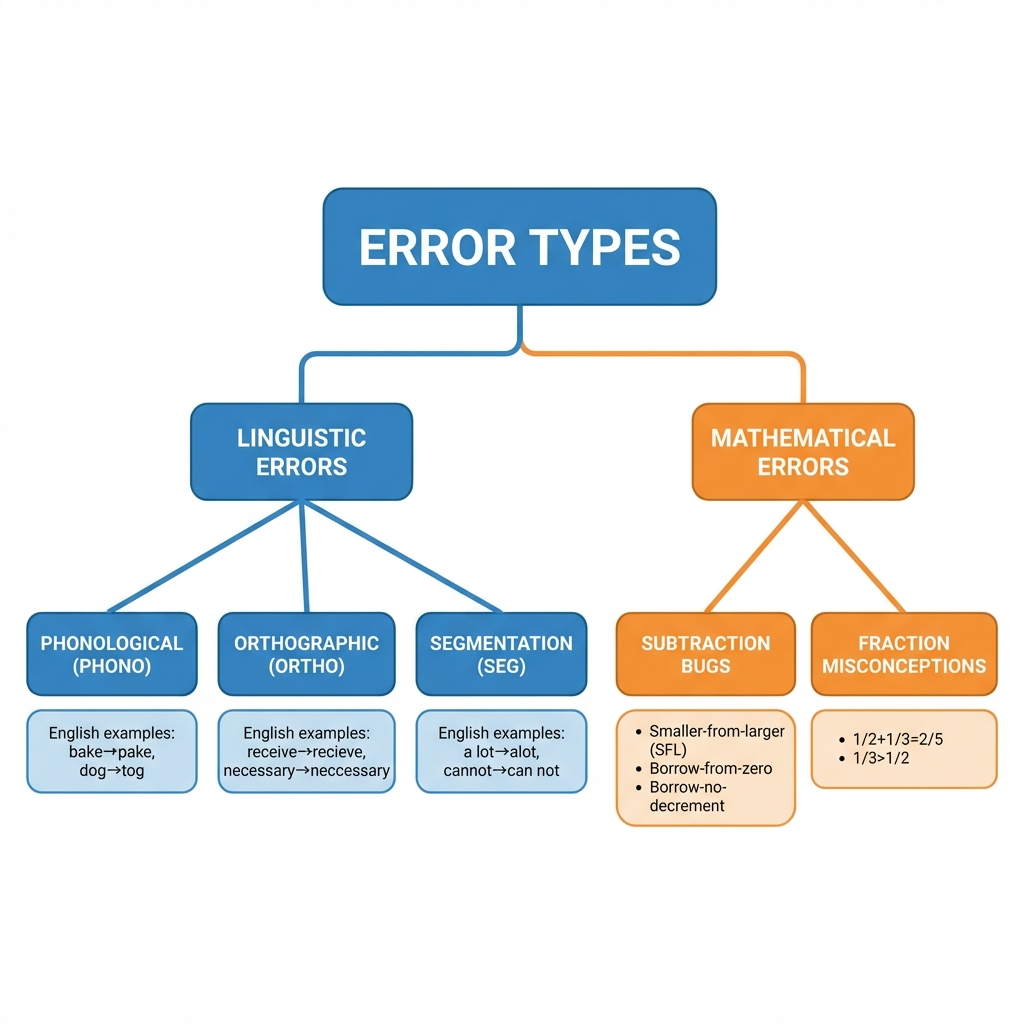
\includegraphics[width=0.9\textwidth]{figures/error_taxonomy.png}
\caption{Hierarchical error taxonomy showing linguistic and mathematical error categories with examples.}
\label{fig:error_taxonomy}
\end{figure}

\subsection{Linguistic Error Categories}
\label{sec:method_tax_ling}

For linguistic errors in typed student text, the taxonomy targets patterns associated with persistent learning difficulties, not general grammatical or typographical errors. Three primary categories are defined.

\textbf{Phonological Errors (ERR-PHONO).} These errors are commonly associated in the learning-difficulty literature with difficulty in phoneme-grapheme conversion, as described in accounts of phonological dysorthography. Observable patterns include:
\begin{itemize}
    \item Voicing substitutions are systematic confusions between voiced and voiceless consonants (e.g., /p/$\leftrightarrow$/b/, /t/$\leftrightarrow$/d/, /f/$\leftrightarrow$/v/, /k/$\leftrightarrow$/g/). Example: ``bato'' for ``pato'', ``gola'' for ``cola''.
    \item Syllable inversions reorder phonemes within words. Example: ``parto'' for ``prato'', ``trota'' for ``torta''.
\end{itemize}

\textbf{Orthographic Errors (ERR-ORTHO).} These errors are commonly associated with difficulty in visual-orthographic memory, where the student struggles to recall correct spellings despite intact phonological processing. Observable patterns include:
\begin{itemize}
    \item Contextual rule violations are errors in context-dependent spelling rules (e.g., ``s'' vs. ``ss'' vs. ``ç'' in Portuguese; ``c'' vs. ``k'' in English). Example: ``caza'' for ``casa''.
    \item Homophone confusions substitute words that sound identical but differ in spelling. Example: ``há'' vs. ``à'', ``their'' vs. ``there'' vs. ``they're''.
\end{itemize}

\textbf{Segmentation Errors (ERR-SEG).} These errors reflect difficulty in word boundary perception. Observable patterns include:
\begin{itemize}
    \item Hyposegmentation is the incorrect joining of words. Example: ``derrepente'' for ``de repente'', ``alot'' for ``a lot''.
    \item Hypersegmentation is the incorrect splitting of words. Example: ``em baixo'' for ``embaixo'', ``to gether'' for ``together''.
\end{itemize}

Classification also depends on the semantic context of the error. For example, ``bato'' is a valid Portuguese word (``I beat''), so detecting it as a phonological error for ``pato'' (``duck'') requires analyzing the surrounding sentence context. This motivates the use of contextual language models (Section~\ref{sec:method_models_ling}).

The taxonomy is operational: each category is defined by an observable surface relationship between the written form and its target (phonetic faithfulness, boundary structure, rule- or homophone-based substitution; the mapping rules are given in Section~\ref{sec:impl_ling_taxmap}). The associations with underlying processing difficulties stated above are motivational, drawn from the learning-difficulty literature; they are not constructs the system measures. The taxonomy itself is language-general; the three categories describe error-production mechanisms, not properties of any particular orthography. The implementation and evaluation in this thesis are English-language, for data-availability reasons discussed in Section~\ref{sec:method_data_sources}; Portuguese examples are retained above because the taxonomy was originally motivated by the Portuguese school context, and Portuguese support is the most valuable direction for future work (Chapter~6).

\subsection{Mathematical Error Categories}
\label{sec:method_tax_math}

For mathematical errors in typed numeric responses, the taxonomy targets systematic procedural misconceptions, not computational slips. Two primary categories are defined, following the ``malrule'' tradition in cognitive modeling \parencite{VanLehn1990,BrownBurton1978}:

\textbf{Subtraction Procedural Bugs (ERR-SUB).} Systematic errors in multi-digit subtraction that reflect incorrect procedural rules, not careless mistakes. Specific bugs include:
\begin{itemize}
    \item In the smaller-from-larger bug (SFL), the student always subtracts the smaller digit from the larger, ignoring column position. Example: $43 - 17 = 34$ (computing $7-3=4$ and $4-1=3$).
    \item In borrow-from-zero, borrowing is handled incorrectly when a zero is present. Example: $302 - 158 = 254$ (treating the zero as 10 without borrowing from the hundreds).
    \item In borrow-no-decrement, the student borrows to the ones column but fails to decrement the tens column. Example: $52 - 27 = 35$ (computing $12-7=5$ but then $5-2=3$).
\end{itemize}

\textbf{Fraction Misconceptions (ERR-FRAC).} Conceptual errors in fraction operations rooted in ``whole-number bias'', the tendency to treat fraction components as independent integers. Specific misconceptions include:
\begin{itemize}
    \item Independent numerator-denominator addition means adding fractions by adding numerators and denominators separately. Example: $\frac{1}{2} + \frac{1}{3} = \frac{2}{5}$.
    \item Magnitude comparison by component means comparing fractions by comparing numerators or denominators independently. Example: claiming $\frac{1}{5} > \frac{1}{3}$ because $5 > 3$.
\end{itemize}

In the buggy-procedure tradition these error patterns are regarded as diagnostically informative, since they reveal a systematically applied incorrect rule rather than an isolated slip, which motivates their early identification \parencite{VanLehn1990}.

\subsection{Label Scheme and Annotation Guidelines}
\label{sec:method_tax_labels}

For linguistic errors, the annotation scheme adopts a token-level or span-level labeling format compatible with sequence-labeling models. The BIO (Begin-Inside-Outside) tagging scheme applies:
\begin{itemize}
    \item \texttt{O}: Token is correct (outside any error span).
    \item \texttt{B-PHONO}: Beginning of a phonological error span.
    \item \texttt{I-PHONO}: Inside a phonological error span.
    \item Similarly for \texttt{B-ORTHO}/\texttt{I-ORTHO} and \texttt{B-SEG}/\texttt{I-SEG}.
\end{itemize}

For mathematical errors, each student response (problem-answer pair) receives a categorical label from the set: \{\texttt{CORRECT}, \texttt{SFL}, \texttt{BORROW\_ZERO}, \texttt{BORROW\_NO\_DEC}, \texttt{FRAC\_ADD}, \texttt{FRAC\_COMPARE}, \texttt{OTHER\_ERROR}\}.

\section{Data Strategy}
\label{sec:method_data}

Data scarcity is the main methodological challenge of this thesis. Corpora of student responses annotated with difficulty-linked error types, for K--12 populations, with per-student longitudinal structure, are almost nonexistent in public form, for the same privacy and ethics reasons (GDPR, data about minors) that make collecting them hard. The thesis treats this as the problem statement behind hypothesis H2, namely whether synthetic data can compensate when real data cannot be obtained at scale. The subsections below document the data sourcing decisions, including the sources that were considered and rejected.

\subsection{Data Source Selection}
\label{sec:method_data_sources}

On language, the project was initially oriented toward Portuguese, the natural deployment context. The best available Portuguese error-annotated resource, the COPLE2 learner corpus \parencite{Mendes2016}, was examined and rejected as a primary source because of a population mismatch. COPLE2 documents adult foreign learners of Portuguese, whose error distribution (interference from the mother tongue, morphosyntax of a second language) differs fundamentally from that of native-speaker children with learning difficulties. Since no Portuguese child-population error corpus was available, and the thesis's research questions do not depend on any particular language, experimentation moved to English, where substantially larger error-annotated corpora exist. This trade of deployment realism for data availability and statistical power is revisited in the limitations (Chapter~5) and future work (Chapter~6).

For real linguistic data, candidate English corpora were assessed against three criteria: error annotations at span level (corrected text alone was not enough), a license obtainable within the project's timeline, and a machine-readable format with an existing parsing ecosystem. The outcome for each corpus follows.
\begin{itemize}
    \item BEA-2019 W\&I+LOCNESS \parencite{Bryant2019} was adopted. It provides gold ERRANT/M2 span annotations, is free for non-commercial research, and can be downloaded directly.
    \item CLC FCE v2.1 \parencite{YannakoudakisBriscoeMedlock2011} was also adopted; it has the same M2 format and license class. It was initially catalogued as requiring signed license paperwork and deferred; a later check found the BEA-2019 release of FCE is directly downloadable, and it was integrated, growing the real training pool by a factor of 2.7 (Chapter~5).
    \item NUCLE/CoNLL-2014 was rejected. It requires signed institutional license agreements with turnaround incompatible with the project timeline, and adds no annotation type the adopted corpora lack.
    \item Lang-8/cLang-8 ($\sim$2.4M sentence pairs) was deferred. It requires a registration process with manual approval, and was identified as the natural scale-up path if the adopted corpora proved insufficient, which the results of Chapter~5 did not indicate.
    \item The Holbrook corpus \parencite{Holbrook1964,Mitton1985} contains writings of 19 schoolchildren with severe literacy difficulties and was adopted for evaluation only. It is the only located public English corpus from (approximately) the target population. With 531 usable sentences it is far too small to train on, but it suits the measurement of domain shift from the adult-learner training corpora to struggling child writers. The Spanish DysList resource \parencite{RelloBaezaYates2014} confirms that dyslexic-error corpora exist for other languages but offers no English data.
\end{itemize}

For mathematics, the original plan used DeepMind's \texttt{mathematics\_dataset} generator as the source of correct base problems for malrule injection. It was discarded during implementation because the package is unmaintained and incompatible with current versions of its own dependencies. The needed problem classes (multi-digit subtraction, fraction pairs) are trivially generatable, so a self-written generator replaced it; a heavyweight external dependency was not worth its maintenance risk for 50 lines of controlled generation code. The MaE dataset of expert-validated algebra misconceptions (MIT license) was retained as reference material for future extension beyond arithmetic. The ASSISTments 2009--10 dataset \parencite{Feng2009Assistments} was examined as a source of math error labels and found unsuitable for that purpose. It records correctness, attempts, and hints, but not \emph{which} procedural bug produced a wrong answer. Those same behavioral signals make it valuable for the profiling module (below), where it was adopted instead.

For profiling, no public dataset offers longitudinal, per-student, difficulty-labeled responses (the GDPR/minors constraint above binds hardest here). The strategy therefore has three parts: (i) a simulator with known ground-truth archetypes, testing whether they can be recovered; (ii) the Holbrook corpus reused at the student level (per-child error distributions), testing whether archetype-like structure exists in real struggling writers; and (iii) ASSISTments (525{,}534 responses, 4{,}217 students), testing whether behavioral profiles are stable per-student traits over real longitudinal histories. None of the three alone would support H3, so the design uses separate data for recoverability, realism, and stability.

\subsection{Rule-Based Synthetic Data Generation}
\label{sec:method_data_rule}

Rule-based generators provide controlled synthetic data with guaranteed label accuracy, because the corruption is injected programmatically and the BIO span labels are therefore correct by construction. Starting from correct sentences, corruption rules inject specific error types:
\begin{itemize}
    \item Phonological errors come from probabilistic substitution of confusable consonant pairs (p/b, t/d, f/v, k/g) and phonetically-faithful respellings, based on documented confusion patterns.
    \item Orthographic errors come from substitution of frequently confused grapheme patterns and homophone swaps.
    \item Segmentation errors come from word fusion (removing spaces) or word splitting (inserting spaces at plausible boundaries).
\end{itemize}

Correct base sentences are drawn from a public Wikipedia-derived sentence corpus, filtered to 5--18 words and plain punctuation ($\sim$600{,}000 sentences). The size of the base pool came from a failure. The first implementation used 20 hand-written template sentences, and the resulting evaluation scores turned out to measure template memorization, not generalization (Chapters~4 and~5 document this failure and its diagnosis). For mathematics, transformation rules apply each malrule to generated problems, recording correct answer, malrule answer, and label; problems where two malrules produce identical answers are filtered out as formally ambiguous (Chapter~4).

\subsection{LLM-Based Synthetic Data Generation: Considered, Not Adopted}
\label{sec:method_data_llm}

Large Language Models were considered as a second synthetic-data source, generating more naturalistic student errors via few-shot prompting. This path was not adopted in the final system, for three reasons weighed against the properties of the rule-based generator:
\begin{enumerate}
    \item Rule-based corruption yields span labels that are correct by construction, whereas LLM-generated errors require post-hoc verification of both the error's type and its exact span. That reintroduces, at scale, the annotation cost the synthetic strategy exists to avoid.
    \item The final training set uses $10^6$ synthetic sentences. Generating at that scale through commercial LLM APIs would have a real cost, while the rule-based generator is free and fast.
    \item The taxonomy's three categories are surface-realizable by rules (substitutions, splits, merges); the added naturalness of LLM text plausibly matters more for error types this thesis does not target (discourse-level, semantic).
\end{enumerate}
LLM generation remains attractive for future work where rules are weakest, that is, generating errors with the distributional signature of a specific population (e.g., mimicking the Holbrook error mix identified in Chapter~5) instead of uniform corruption.

\subsection{Data Splits and Validation}
\label{sec:method_data_splits}

The synthetic and real pools are partitioned into training and evaluation splits (90/10). To assess the effect of synthetic data (H2), experiments compare models trained on synthetic data only, real data only, and combined data. Because the curriculum stages are chained (each stage continues from the previous checkpoint; Section~\ref{sec:impl_ling_training}), the real-only comparison point for H2 is a separate model trained on the real pool alone, from the pretrained encoder, with no synthetic stage (Section~\ref{sec:eval_ling_scratch}). One protocol rule, learned the hard way (Chapter~5), is that all claims about real-data performance are measured on all-real evaluation sets, and two additional benchmarks (FCE test; Holbrook) are held out from training entirely.

\section{Proposed Methods}
\label{sec:method_models}

The methods below cover error detection, linguistic and mathematical, and the aggregation of detected errors into student difficulty profiles.

\subsection{Linguistic Error Detection: NLP Sequence Labeling}
\label{sec:method_models_ling}

Linguistic error detection is framed as a sequence-labeling problem, where each token in the input text is assigned an error-type label (or \texttt{O} for correct) \parencite{MaHovy2016,ReiYannakoudakis2016}. This framing was chosen over the sequence-to-sequence formulation dominant in grammatical error correction. The thesis needs to detect and categorize error spans, not rewrite the text, and tagging formulations are cheaper to train and directly interpretable per token \parencite{Omelianchuk2020GECToR}.

The architecture is a pretrained Transformer encoder fine-tuned for token classification, with three parts.
\begin{itemize}
    \item The encoder is a pretrained language model; candidates included BERT, RoBERTa, XLM-RoBERTa (for future multilingual work) and DeBERTa-v3. The final selection (DeBERTa-v3-base) and its rationale are given in Chapter~\ref{chap:Chapter4}.
    \item The classification head is a linear layer mapping each token's contextual embedding to the label space (\texttt{O}, \texttt{B-PHONO}, \texttt{I-PHONO}, \texttt{B-ORTHO}, \texttt{I-ORTHO}, \texttt{B-SEG}, \texttt{I-SEG}).
    \item Training uses a token-level classification loss. The label distribution is severely imbalanced (most tokens are correct), and the choice of loss function turned out to be one of the hardest implementation problems of the thesis; Chapter~\ref{chap:Chapter4} documents the full progression (plain cross-entropy, weighted variants, focal loss) with the observed failure of each intermediate step.
\end{itemize}

Pretrained Transformers use subword tokenization, which typically splits misspelled words differently from correct words. Error labels are assigned to the first subword of each token, with subsequent subwords receiving a continuation label or being ignored during evaluation.

Contextual models can distinguish legitimate words from contextual errors. For example, ``bato'' is correctly predicted as an error in ``O bato nada'' (intended: ``O pato nada'') but not in ``Eu bato à porta'' (correct usage).

\subsection{Mathematical Error Detection: Symbolic and ML Methods}
\label{sec:method_models_math}

Mathematical error detection uses the structured nature of arithmetic problems and deliberately implements two contrasting methods, since their comparison is itself a research question (Q3).

The symbolic method is malrule simulation. For each known misconception (SFL, borrow-from-zero, etc.), a procedural simulation computes what result the student would produce if applying that malrule. The student's actual response is compared against the correct answer and each malrule's predicted answer; an exact match assigns the label. This method is exact and interpretable by construction and, by the same construction, intolerant to any deviation from the modeled procedure.

The second method is a feature-based ML classifier: a gradient-boosted decision tree classifier over hand-built numeric features of the (problem, answer) pair, trained on generator output. The initial plan called for this classifier only as an optional disambiguator; it was promoted to a co-equal method during implementation, both because the thesis's research questions explicitly compare symbolic and ML approaches and because early experiments showed the two methods fail in complementary ways (exactness versus robustness, quantified in Chapter~5).

\subsection{Active Screening vs.\ Passive Monitoring}
\label{sec:method_models_screening}

The system distinguishes two acquisition regimes for linguistic errors, routed to different detection methods.

\textbf{Passive monitoring (open world).} In free writing, the intended words are unknown; detecting an error requires inferring both that a span is wrong and what was meant. Only a learned contextual model can solve this inference problem. It is where the neural sequence labeler operates, and where its training-population dependence matters.

\textbf{Active screening (closed world).} In a designed worksheet item (dictation of a target word; an arithmetic problem), the correct answer is known in advance. Error classification then reduces to comparing the written form against the known target through the same deterministic taxonomy logic used to build the corpora, with no model inference and no training-population dependence. The cost is coverage, since screening only observes the items it poses.

The closed-world regime has a second advantage, \emph{item selection}. Each screening item is chosen to maximize the diagnostic information of the error it may elicit: irregularly-spelled but phonetically recoverable words isolate the orthographic-memory profile; short regular words isolate phoneme-grapheme conversion; compounds isolate word segmentation; and arithmetic items are admitted only if every modeled malrule yields a distinct answer (the distinguishability policy of Chapter~5). This is the same principle as classical diagnostic test design, applied programmatically. The two regimes are complementary by design. Screening is intended to yield high-information signal from one or two worksheets and, having no trained component, does not depend on any training population (it does depend on the item bank and on the mapper's rules); monitoring accumulates broad-coverage signal over time.

\subsection{Student Difficulty Profiling: Clustering and Aggregation}
\label{sec:method_models_profile}

Error detection produces per-response labels. To identify persistent difficulty patterns, errors are aggregated across multiple responses per student and analyzed for stability.

For each student, an error profile vector is constructed from the proportion of each error type among the student's errors, the overall error rate, and the temporal trend of errors across sessions. The overall rate is included alongside the proportions because proportion-only vectors are provably blind to profiles that differ in error frequency but not error mix; Chapter~4 documents this defect, which was found empirically in simulation.

Clustering uses KMeans (fixed $k$, swept by silhouette) and HDBSCAN \parencite{Campello2013HDBSCAN} (no fixed $k$, native outlier handling, which matters because students with atypical profiles are exactly the interesting cases in this application). Hierarchical clustering and plain DBSCAN were considered; HDBSCAN subsumes the practical advantages of both for this use case.

Cluster centroids are examined to identify the characteristic error pattern of each group (e.g., ``phonological-dominant''). Interpretability is assessed by centroid inspection against the taxonomy; validation with practicing educators is planned as part of the future school pilot (Chapter~6), not claimed here. Throughout the thesis, ``difficulty profile'' denotes such a statistical profile over observable error patterns; it is not a measurement of an underlying cognitive or clinical construct (Section~\ref{sec:eval_discuss_threats}).

Where longitudinal data is available, error recurrence is analyzed: a profile is considered stable if the same error types persist across multiple sessions, distinguishing persistent difficulties from episodic mistakes.

\section{Evaluation Framework}
\label{sec:method_eval}

Each component of the system is evaluated with the metrics and protocols specified in the subsections below.

\subsection{Error Detection Metrics}
\label{sec:method_eval_detect}

For linguistic error detection (sequence labeling), evaluation uses span-level metrics computed with seqeval:
\begin{itemize}
    \item Precision is the fraction of predicted error spans that exactly match gold spans (boundary and type).
    \item Recall is the fraction of gold error spans that are exactly predicted.
    \item The $F_1$-score is the harmonic mean of precision and recall.
\end{itemize}

Span-level scoring with exact boundaries is deliberately strict; it understates partial credit but cannot be gamed by over-flagging. Metrics are reported per benchmark; per-error-type breakdowns and predicted-tag distributions are inspected diagnostically (a model collapsing to a single class is visible in the distribution but not in aggregate $F_1$).

For mathematical error detection, evaluation uses classification metrics: accuracy, macro-$F_1$ over error classes, and confusion analysis for systematic misclassifications.

\subsection{Clustering Metrics}
\label{sec:method_eval_cluster}

For student difficulty profiling, clustering quality is assessed using:
\begin{itemize}
    \item The silhouette coefficient \parencite{Rousseeuw1987} measures cluster cohesion and separation, and is used for internal quality and $k$ selection.
    \item The Adjusted Rand Index \parencite{HubertArabie1985} measures agreement with ground truth where it exists (simulation), and agreement between independent re-clusterings where it does not (split-half stability on real data).
    \item The Davies--Bouldin index \parencite{DaviesBouldin1979} is a secondary internal-quality check.
\end{itemize}

\subsection{Synthetic vs. Real Data Comparison}
\label{sec:method_eval_synth}

To assess the effectiveness of synthetic data (H2), experiments compare performance on held-out real test data when training on synthetic-only, real-only (from scratch), and combined data. Two protocol rules apply, both introduced after evaluation-design failures documented in Chapter~5. Evaluation splits must not share base material with training data (the template-memorization incident), and mixed-composition evaluation sets must not be used for real-data claims (the synthetic-dominated-eval incident).

\section{Tools and Implementation}
\label{sec:method_tools}

The implementation uses Python (3.10--3.12); PyTorch and Hugging Face Transformers for the neural model; ERRANT's M2 format and parsing conventions \parencite{BryantFeliceBriscoe2017} for real GEC data; seqeval for span-level scoring; scikit-learn \parencite{Pedregosa2011} for the gradient-boosted classifier, clustering, and metrics; jellyfish (Metaphone \parencite{Philips1990}) for phonetic matching in the taxonomy mapper; a purpose-built European Portuguese grapheme-to-phoneme comparator for the Portuguese screening instantiation (Chapter~4); and Flask with SQLite for the pilot prototype (Chapter~4). Sentence-BERT and \texttt{pyspellchecker} appear only in the proof of concept (Section~\ref{sec:method_poc}). The final system lives in the \texttt{System} directory of the project repository; the POC is preserved separately under \texttt{Experimentation}.

\section{Initial Proof of Concept}
\label{sec:method_poc}

Before the full implementation, an initial Proof of Concept (POC) was developed to validate the feasibility of automated error pattern detection. The POC architecture and results are summarized below, together with the reasons its approach was not carried forward as the core of the final system.

\subsection{POC Architecture}
\label{sec:method_poc_arch}

The POC implements a heuristic-based detection pipeline.

Preprocessing consists of normalization (lowercase, whitespace cleaning) and tokenization of the input text (student answer and reference answer).

Feature extraction then computes three parallel feature streams:
\begin{itemize}
    \item For semantic similarity, Sentence-BERT embeddings (model: \texttt{all-MiniLM-L6-v2}) are computed for both reference and student answers, and cosine similarity is calculated.
    \item For keyword analysis, keywords are extracted from the reference answer, and coverage (fraction of keywords present in student answer) is computed.
    \item For linguistic analysis, spelling errors are counted using \texttt{pyspellchecker}.
\end{itemize}

The heuristic detector is a priority-based decision tree that classifies each answer:
\begin{enumerate}
    \item If semantic similarity $\geq 0.75$ and keyword coverage $\geq 50\%$: classify as \texttt{correct}.
    \item If word count $< 5$: flag as \texttt{vague\_answer}.
    \item If spelling errors $\geq 3$: flag as \texttt{linguistic\_error}.
    \item If semantic similarity $< 0.55$: flag as \texttt{conceptual\_error}.
    \item If keyword coverage $< 40\%$: flag as \texttt{missing\_key\_concepts}.
    \item If no issues detected: classify as \texttt{correct}.
\end{enumerate}

The system selects the highest-confidence issue and generates a human-readable explanation.

\subsection{POC Results}
\label{sec:method_poc_results}

The POC was evaluated on a synthetic dataset of 42 English student answers across three science questions (photosynthesis, water cycle, mitosis/meiosis). Error labels were manually assigned.

Performance was as follows.
\begin{itemize}
    \item Overall accuracy: 66.7\% (28/42 correct predictions)
    \item Linguistic errors: 100\% precision, 100\% recall
    \item Vague answers: 100\% precision, 100\% recall
    \item Conceptual errors: 9\% recall (frequently confused with \texttt{missing\_key\_concepts})
\end{itemize}

\subsection{From POC to Full System: What Was Kept and What Was Replaced}
\label{sec:method_poc_future}

The POC validated the core premise that error patterns, as well as correctness, are automatically detectable. Four of its properties, however, disqualified its approach as the core of the final system, and each drove a concrete design decision:

\begin{itemize}
    \item Response-level flags cannot support the taxonomy. The POC classifies whole answers, but the difficulty taxonomy requires knowing which words are wrong and how. This motivated the token-level sequence-labeling formulation (Section~\ref{sec:method_models_ling}).
    \item A spell-checker cannot separate PHONO from ORTHO from SEG. \texttt{pyspellchecker} counts out-of-vocabulary words, whereas the taxonomy's categories depend on the relationship between the misspelling and its target (phonetic faithfulness, boundary structure). This motivated the taxonomy mapper and the learned model.
    \item Fixed thresholds do not generalize. The POC's similarity cut-offs were tuned to 42 examples and its conceptual-vs-missing confusion (9\% recall) showed heuristics saturating. This motivated learned models trained on orders of magnitude more data.
    \item Single-response classification cannot see persistence. Difficulty is a longitudinal construct, and the POC has no notion of a student. This motivated the profiling module.
\end{itemize}

The POC's conceptual/missing-concepts error categories (science-content errors) were deliberately dropped: they concern subject-matter knowledge, not the difficulty-linked mechanical patterns this thesis targets. The POC code is preserved under \texttt{Experimentation} as a baseline and historical record.

\section{Summary}
\label{sec:method_summary}

This chapter covered the following.
\begin{enumerate}
    \item Error taxonomies for linguistic (phonological, orthographic, segmentation) and mathematical (subtraction bugs, fraction misconceptions) errors, grounded in learning-difficulty research.
    \item A data strategy built around documented sourcing decisions: English over Portuguese (population-mismatch of the available Portuguese corpus), BEA-2019+FCE as real training data, Holbrook as a target-population evaluation benchmark, rule-based synthetic generation at the million-sentence scale (LLM generation considered and rejected with stated reasons), and a three-way profiling evidence design (simulation, real archetypes, real stability).
    \item Detection methods: NLP sequence labeling for linguistic errors, and two deliberately contrasted mathematical methods (symbolic simulation and a gradient-boosted classifier).
    \item Profiling methods: clustering of per-student error vectors, with explicit attention to feature-representation limits and outlier handling.
    \item An initial POC (66.7\% accuracy, heuristic) whose specific failure modes (response-level granularity, undifferentiated spelling detection, threshold brittleness, no longitudinal view) directly motivated the design decisions of the final system.
\end{enumerate}

The following chapters present the implementation and its engineering decisions (Chapter~4), experimental results (Chapter~5), and conclusions (Chapter~6).
